\documentclass[]{article}
\usepackage{lmodern}
\usepackage{amssymb,amsmath}
\usepackage{ifxetex,ifluatex}
\usepackage{fixltx2e} % provides \textsubscript
\ifnum 0\ifxetex 1\fi\ifluatex 1\fi=0 % if pdftex
  \usepackage[T1]{fontenc}
  \usepackage[utf8]{inputenc}
\else % if luatex or xelatex
  \ifxetex
    \usepackage{mathspec}
  \else
    \usepackage{fontspec}
  \fi
  \defaultfontfeatures{Ligatures=TeX,Scale=MatchLowercase}
\fi
% use upquote if available, for straight quotes in verbatim environments
\IfFileExists{upquote.sty}{\usepackage{upquote}}{}
% use microtype if available
\IfFileExists{microtype.sty}{%
\usepackage{microtype}
\UseMicrotypeSet[protrusion]{basicmath} % disable protrusion for tt fontshttps://de.overleaf.com/project/5e85b0680d0bed00011ea790
}{}
\usepackage[margin=1in]{geometry}
\usepackage{hyperref}
\hypersetup{unicode=true,
            pdftitle={The dating of the Human-Neandertal introgression event estimated from present-day human genomes is compatible with a multitude of admixture durations},
            pdfauthor={Leonardo Nicola Martin Iasi (Max Planck Institute for Evolutionary Anthropology, MPI EVA), Dr.~Benjamin Marco Peter (MPI EVA, benjamin\_peter@eva.mpg.de)},
            pdfborder={0 0 0},
            breaklinks=true}
\urlstyle{same}  % don't use monospace font for urls
\usepackage{natbib}
\bibliographystyle{plainnat}
\usepackage{graphicx,grffile}
\makeatletter
\def\maxwidth{\ifdim\Gin@nat@width>\linewidth\linewidth\else\Gin@nat@width\fi}
\def\maxheight{\ifdim\Gin@nat@height>\textheight\textheight\else\Gin@nat@height\fi}
\makeatother
% Scale images if necessary, so that they will not overflow the page
% margins by default, and it is still possible to overwrite the defaults
% using explicit options in \includegraphics[width, height, ...]{}
\setkeys{Gin}{width=\maxwidth,height=\maxheight,keepaspectratio}
\IfFileExists{parskip.sty}{%
\usepackage{parskip}
}{% else
\setlength{\parindent}{0pt}
\setlength{\parskip}{6pt plus 2pt minus 1pt}
}
\setlength{\emergencystretch}{3em}  % prevent overfull lines
\providecommand{\tightlist}{%
  \setlength{\itemsep}{0pt}\setlength{\parskip}{0pt}}
\setcounter{secnumdepth}{0}
% Redefines (sub)paragraphs to behave more like sections
\ifx\paragraph\undefined\else
\let\oldparagraph\paragraph
\renewcommand{\paragraph}[1]{\oldparagraph{#1}\mbox{}}
\fi
\ifx\subparagraph\undefined\else
\let\oldsubparagraph\subparagraph
\renewcommand{\subparagraph}[1]{\oldsubparagraph{#1}\mbox{}}
\fi

%%% Use protect on footnotes to avoid problems with footnotes in titles
\let\rmarkdownfootnote\footnote%
\def\footnote{\protect\rmarkdownfootnote}

%%% Change title format to be more compact
\usepackage{titling}

% Create subtitle command for use in maketitle
\providecommand{\subtitle}[1]{
  \posttitle{
    \begin{center}\large#1\end{center}
    }
}

\setlength{\droptitle}{-2em}

  \title{The dating of the Human-Neandertal introgression event estimated from present-day human genomes is compatible with a multitude of admixture durations}
    \pretitle{\vspace{\droptitle}\centering\huge}
  \posttitle{\par}
    \author{Leonardo Nicola Martin Iasi (Max Planck Institute for Evolutionary
Anthropology, MPI EVA), Benjamin Marco Peter (MPI EVA,
\href{mailto:benjamin_peter@eva.mpg.de}{\nolinkurl{benjamin\_peter@eva.mpg.de}})}
    \preauthor{\centering\large\emph}
  \postauthor{\par}
      \predate{\centering\large\emph}
  \postdate{\par}
    \date{2020-09-30}

\usepackage{setspace}
\doublespacing
\usepackage[none]{hyphenat}
\usepackage{amsfonts}
\usepackage{amssymb}
\usepackage{graphicx}
\usepackage{float}
\usepackage{xcolor}
\floatplacement{figure}{H}

\begin{document}
\maketitle

\section{Abstract}\label{abstract}

\section{Introduction}\label{introduction}



\subsection{(Archaic) Interbreeding, genomic consequences and why is it interesting}\label{(Archaic) Interbreeding, genomic consequences and why is it interesting}

The sequencing of Neandertal \citep{green_draft_2010,prufer_complete_2013,prufer_high-coverage_2017, mafessoni_high_coverage_2020} and Denisovan genomes \citep{reich_genetic_2010, meyer_high-coverage_2012} revealed that modern humans outside of Africa interacted, and admixed with these archaic hominins \citep{vernot_resurrecting_2014,fu_genome_2014,fu_early_2015,sankararaman_genomic_2014,sankararaman_combined_2016,vernot_excavating_2016,malaspinas_genomic_2016}. There are two major lines of evidence: First, Neandertals are genome-wide more similar to non-Africans than to Africans \citep{green_draft_2010, meyer_high-coverage_2012}. This shift can be explained by 2-4\% of admixture from Neandertals into non Africans \citep{green_draft_2010, prufer_complete_2013}. Similarly, East Asians and Papuans are more similar to Denisovans \citep{meyer_high-coverage_2012} than other human groups, which is likely due to gene flow from Denisovans. 

As a second line of evidence, all non-Africans carry genomic segments that are very similar to the sequenced archaic genomes. As these putative \emph{admixture segments} are up to several hundred kilobases (kb) in length, they are unlikely to predate the split of modern humans from Neandertals and Denisovans \citep{sankararaman_genomic_2014, vernot_resurrecting_2014}. Rather, they entered the modern human populations later through gene flow \citep{sankararaman_date_2012, sankararaman_combined_2016, vernot_excavating_2016, skov_detecting_2018, skov_nature_2020}. 

\paragraph{Why do we care about timing of gene flow}.

One open question is when and where this gene flow happened. This is important because it potentially constrains some major events in human genetic history pertaining to the interactions between Neandertals and modern humans in Eurasia that led to the eventual replacement of Neandertals. In particular, as no Neandertals have been found in Africa, the first Out-Of-Africa event is likely the earliest time point where humans and Neandertals could have met. Similarly, gene flow must end with the disappearance of Neandertals. As the earliest modern human remains outside of Africa are dated to around 188 thousand years ago (kya)  \citep{stringer_when_2018,hershkovitz_earliest_2018} and the latest Neandertals are suggested to be between 37 kya and 39 kya old \citep{zilhao_precise_2017, higham_timing_2014}. This leaves a potential time frame for Neandertal and modern human interaction of well over 140,000 years. However, direct evidence of modern humans and Neandertals in the same geographical location at the same time is much spottier; in Europe, for example Neandertals and modern humans likely overlapped only for less than 10,000 years \citep{bard_extended_2020}. Thus, detailed genetic dating of when Neandertals and modern human admixture started and ended could help making the dating of these events more precise.

\subsection{Admixture segment models}\label{Admixture models}

The most common approach to admixture dating is using a ``recombination clock'': Conceptually, admixture segments are the result of recombination breaking down introduced chromosomes: The offspring of an archaic and modern human parent will have full chromosomes of either ancestry. If this individual has offspring in a largely modern human population, meiotic recombination progressively breaks the ancestry segments of the archaic chromosome  down into smaller and smaller pieces, whose size decrease with time \citep{falush_inference_2003, liang_lengths_2014, gravel_population_2012}. Correspondingly, one would expect the segments of Neandertal ancestry in early modern human specimens to decrease with time, a signal that has been recovered consistently from early modern human genomes \citep{fu_genome_2014, moorjani_genetic_2016, sikora_ancient_2017, sikora_population_2019}. 

\subsection{Inference}
Models to infer the admixture time thus exploit this inverse relationship between admixture time and segment length for inference of the  the time of an admixture event \citep{moorjani_history_2011,pugach_dating_2011,sankararaman_date_2012,loh_inferring_2013,sankararaman_combined_2016,pugach_gateway_2018,jacobs_multiple_2019,hellenthal_genetic_2014,pool_inference_2009,moorjani_history_2011,gravel_population_2012,liang_lengths_2014}. The simplest models assume that admixture segments are rare and inbreeding is not significant, such that admixture segments are unlikely to recombine with each other \citep{pool_inference_2009,liang_lengths_2014}. Further assumptions are that the segments act neutrally \citep{shchur_distribution_2019} and the recombination rate is the same in different populations at all times \citep{gravel_population_2012}. In addition, it is frequently assumed that the admixture happens over a very short time period, in a single \textit{admixture pulse} \citep{moorjani_history_2011}, usually modelled as a single generation of gene flow.


\subsection{The two approaches and their application to find archaic admixture dates}\label{the-two-approaches-and-their-application-to-find-archaic-admixture-dates}

The first step in dating admixture events from genetic data is therefore estimating the length distribution of admixture segments.  There are two main approaches for this; a first sets of methods starts with identifying all admixture segments over a certain length, and then use the length distribution of these segments for inference. Alternatively, the length distribution can also be estimated from patterns of linkage along a chromosome directly, without explicitly inferring the genomic location of these segments (\citep{chimusa_dating_2018}) (Figure \ref{fig:fig1} B).

 In the first set of approaches, the identification of segments is largely independent from the later dating, and can be done using a variety of methods \citep{racimo_signatures_2017,seguin_orlando_paleogenomics_2014,vernot_excavating_2016,sankararaman_combined_2016,skov_detecting_2018}. These approaches are most useful for recent admixture estimated on high-quality data, as uncertainty in the segment identification is not easily fed forward into the timing inference \citep{hellenthal_genetic_2014}.

Thus, methods using admixture-induced linkage disequilibrium (ALD) are more widely used \citep{moorjani_history_2011,sankararaman_date_2012,sankararaman_combined_2016}. As admixture introduces entire chromosomes, variants that result from the differences between the parental chromosomes are all in linkage disequilibrium (LD) \citep{chakraborty_admixture_1988,stephens_mapping_1994,wall_detecting_2000}. As recombination decreases the size of admixture segments over time, the linkage decreases correspondingly \citep{patterson_methods_2004}. 

In case of a recent admixture event a few tens of generations ago, ALD stretches  over long genetic distances and is therefore easily distinguishable from short range LD due to inheritance of chromosomal segments from an ancestral population, or LD caused by bottlenecks and genetic drift after the split from the parental populations \citep{moorjani_history_2011}. For ancient admixture events however, ALD is quite similar to the genomic background. To partially circumvent this issue for dating the Neandertal-human admixture time, variants are ascertained such that only  markers that are (nearly) differentially fixed between the two groups are used 
\citep{sankararaman_date_2012}. 

Typically, estimation of admixture dates proceeds by fitting a decay curve of pairwise LD as a function of genetic distance, using an exponential distribution whose parameter is informative for the time of an admixture pulse \citep{moorjani_history_2011,loh_inferring_2013}. 



\subsection{What is known about admixture}

Using this approach, Sankararaman et al. dated the Neandertal-human admixture pulse to be  between 37--86 kya (most likely range of 47–65 kya)  \citep{sankararaman_date_2012}. Later, this date was refined to 41 kya -- 54 kya (95\% CI) using a different ascertainment scheme combined with a different genetic map for European populations \citep{moorjani_genetic_2016}. A date of 50 -- 60 kya was obtained from the analysis of the \textit{Ust-Ishim} early modern human from Siberia \citep{fu_genome_2014}.

Using D-statistics \citep{green_draft_2010} and by directly inferring introgressed segments, it was found that the amount of Neandertal ancestry is 24\% higher in present-day East-Asians compared to Europeans \citep{meyer_high-coverage_2012 ,  wall_higher_2013}. A second admixture event private to East-Asians around the same time as the interbreeding event between Neandertals and all non-Africans is suggested to explain the higher amount of ancestry \citep{kim_selection_2015,vernot_complex_2015}.

Compared to the relatively simple patterns of inference in Neandertal ancestry, Denisovan ancestry in modern humans is more complex. Among present-day populations, Papuans and Melanesians have the highest amount of Denisovan ancestry (6\%), much more than East-Asians (0.2\%) \citep{reich_genetic_2010,meyer_high-coverage_2012}.
However, the Denisovan ancestry segments in East Asians are made up of two distinct groups, one from a population only distantly related to the sequenced Denisovan genome, and another one that is more closely related \citep{browning_analysis_2018}. In contrast, Papuans and Melanesians only have segments from the first of this group, despite them having much more overall ancestry.
One explanation is that there has been a common admixture event into an ancestor of both populations, and a second event that only contributed to East Asians; however the admixture fragment lengths of these two sets of populations are not significantly different from each other, suggesting either a lack of power to distinguish the two events by time, or that they occurred roughly at the same time\citep{browning_analysis_2018}.



The evidence for more complex patterns of Neandertal gene flow is more spotty, as most Neandertal admxiture segments have a similar divergence to the sequenced Neandertals \cite{browning_analysis_2018}. However, several examples of  Neandertal gene flow private to a local population is the identification of admixture segments spanning several Mbp in \textit{Oase 1}, the genome of an early modern human from Romania. He had a recent Neandertal ancestor less than 200 years before he lived (~37–42 kya). (, later than the age of the \textit{Ust'Ishim} modern human which is already admixed with Neadertals. \textit{Oase 1} did however not contribute substantially to present-day human populations  \citep{fu_genome_2014,fu_early_2015}.)


\subsection{Limitations of the pulse model}\label{Why can't we us the pulse model}

The admixture pulse model used in most dating method assumes that gene flow occurs over a short time period; however it is currently unclear how short a time period would be consistent with an admixture pulse model. This is problematic because admixture time estimates under a pulse model may be hard to interpret, as some gene flow could have happened tens of thousands of years before or after the estimated time point.



\subsection{Previous attempts of a general admixture model and ours}\label{Previous attempts of a general admixture model and ours}

To address this issue, the simple pulse model can be extended to include  multiple admixture pulses. The distribution of admixture track lengths will then be a mixture of the exponential distributions from each constituent pulses. This is especially useful if the events are very distinct in time, e.g. if one event is only a few generations back, and the other pulse occurred hundreds of generations ago \citep{fu_genome_2014,slon_genome_2018}. In this case, the admixture segments will be either very long if they are recent, or much shorter if they are older. It is also very useful if the two admixing sources are very distinct from each other, so that distinct sources can be distinguished. 

Zhou et al. 2017 \citep{zhou_modeling_2017} showed that this model, in principle, can be used for continuous mixtures as well, using a polynomial function as a mixture density. However, they found that even for relatively short admixture events, the large number of parameters led to an underestimate of admixture duration \citep{zhou_inference_2017}, and the beginning and end of admixture were not well inferred
\citep{zhou_modeling_2017,zhou_inference_2017}. 

Ralph and Coop 2013 used the distribution of shared identical by descent (IBD)  segments length between pairs of individuals to infer the number and age of genetic common ancestors. By modeling over all ancestor and ages they fit more complex migration patterns. However, a major problem they found is that a large set of migration patterns fit the IBD distribution equally well. To coup with this they introduced a regularization scheme to their likelihood function by adding a penalization term \citep{ralph_geography_2013}.

\paragraph{Extended Pulse Model}
One drawback of  these approaches are that they introduce a large number of parameters. Even a discrete mixture of two pulses requires at least three parameters (two times and the relative magnitude of the two events) \citep{pickrell_ancient_2014}, and the more complex models require regularization schemes for fitting.

Here, we present the \emph{extended admixture pulse} model (Figure \ref{fig:fig1} A) to estimate the duration of an admixture event. It only adds one additional parameter, reflecting the duration of gene flow, while retaining much of the mathematical simplicity present in the simple pulse model. 
The extended pulse model assumes that migration rate over time is Gamma distributed, so that the  distribution of admixture segment lengths has a closed form (Figure \ref{fig:fig1} C \& D) with mean admixture time and duration as the two parameters.

Conceptually, identifying an extended pulse model requires us to establish that the length distribution of introgressed segments deviates from an exponential distribution. However, other biases, such as the demography of the admixed population, the accuracy of the recombination map and the ascertainment scheme may also introduce similar signals. Thus, we have to carefully evaluate potential sources of biases  \citep{sankararaman_date_2012,fu_genome_2014,moorjani_genetic_2016}. 


\subsection{What we want to do}\label{what-we-want-to-do}

Here, we first formally define the extended admixture pulse model and derive the resulting segment length distribution. We then introduce inference schemes, either based directly on inferred segment lengths or by using the ALD decay. 
We then use simulations under the extended pulse model to assess the effect of ongoing admixture on inference done under the simple pulse model, and investigate under which scenarios we can distinguish between the two models. We show that while very recent events can be distinguished, for the parameter regions relevant for the  case of archaic admixture, simple pulses cannot be distinguished from more continuous admixture events. Using the 1000 Genomes data, ALD inferred admixture times from Europeans are consistent with a multitude of duration times.
We conclude that while current methods are sufficient to estimate the mean admixture time, these estimates are consistent with gene flow that may have spanned several tens of thousands of years, thus limiting the interpretability of these results. Leaving the question when gene flow happened unsuitable to estimate the duration of admixture and thus answer when the contact between Neandertals and modern humans started or ended.

\begin{figure}
\centering
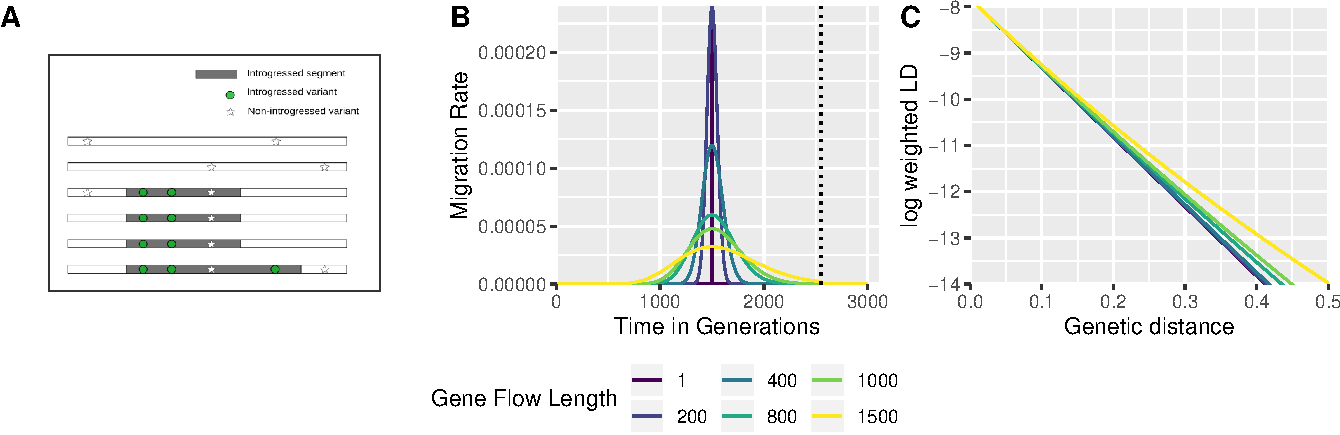
\includegraphics{Admixture_Time_Inference_Paper_Draft_files/figure-latex/fig1-1.pdf}
\caption{\label{fig:fig1} A) Neandertal introgression into non-Africans with a multitude of potential admixture durations. B) The time and duration of admixture results in different length distributions of introgressed chromosomal segments (grey) containing  Neandertal variants (green circles)  in high LD to each other
compared to the background . The ALD approach estimates linkage
between the introgressed variants (green circles), wheres the haplotype approach tries
to estimate the segment directly (grey area). C) Migration rate per generation
modeled using the extended pulse model for different admixture durations (colored lines). The filled area under the curve indicates the discreat realization of the duration of gene flow $t_d$.
The dotted line indicates the maximum time of gene flow. D) The expected LDdecay under the extended pulse model.}
\end{figure}

\section{Methods}\label{methods}
In this section,  we introduce the extended admixture pulse model as a generalization of a more simple single pulse model, and introduce inference algorithms for fitting the extended admixture pulse model to ALD and segment data. 

We then present the details on the simulation settings we use to evaluate these models.

We use these simulations to assess the performance of inference methods assuming the simple pulse model under more complex admixture scenarios, and test the impact of technical variables such as recombination rate variation or demographic scenarios and evaluate when the two models can be distinguished.

Finally, we apply our methods to distinguish several admixture scenarios with different durations to ALD data from the 1000 Genomes Project \citep{the_1000_genomes_project_consortium_global_2015} with 3 high coverage Neandertals \citep{prufer_complete_2013,prufer_high-coverage_2017,mafessoni_high_coverage_2020}.


\subsection{Admixture Models and Inference}\label{admixture models}

In this section, we present formal definitions of the admixture models used.  We assume we have $n$ admixture segments. We denote the length of the $i$-th segment as $L_i$. Further, the random variable $T_i$ represents the time when fragment $L_i$ entered the population. We assume that the $L_i$ and $T_i$ are both realizations from more general distributions $L$ and $T$ that reflect the overall segment length and admixture time distributions, respectively. 

Given $T_i$, we assume that $L_i$ is exponentially distributed with rate parameter given by the admixture time $t_a$ and the recombination rate $r$.
\begin{equation}
\label{eq:generall_length_distribution}
    P(L_i=l|T_i=t) = t r\exp{-t r l} 
\end{equation}

If we measure the length of each segment $L_i$ in the recombination distance Morgan (M), $r=1$ and is omitted from this section for simplicity.

We assume that  $T_i$ is drawn from a distribution $T$. In that case, we need to integrate over all possible values of $T_i$. 

\begin{equation}
\label{eq:standard_likelihood_definintion}
    P(L_i=l)=\int_{0}^{\infty} P(T_i=t) P(L_i=l | T_i=t) \ dt \text{,}
\end{equation}


Thus, the distribution of the admixture times $T_i$ can be thought of as the mixture density for the exponential mixture of segment lengths $L_i$. 

\subsubsection{The Simple Pulse Model}\label{The Simple Pulse Model}


In the simple pulse model, we assume that all fragments enter the population at the same time $t_m$. Therefore all $T_i$ have the same value $t_m$, and $T$ thus is a constant distribution. We can formalize this by using a Dirac delta function:

\begin{equation}
\label{eq:RV_simple_pulse}
  P(T_i)=\delta_{t_m}(T_i),
\end{equation} 
which integrates to one if $T_i = t_m$.


Therefore,

\begin{equation}
\begin{split}
\label{eq:Likelihood_function_simple_pulse}
    P(L_i=l) &= t_me^{-t_m l}
\end{split}
\end{equation}

The expected segment length under a simple pulse model is given by,

\begin{equation}
\label{eq:Expected_l_simple_pulse}
    \mathbb{E}[L]=\frac{1}{t_m}
\end{equation}

and variance
\begin{equation}
\label{eq:Expected_l_simple_pulse}
    \text{Var}[L]=\frac{1}{t_m^2}
\end{equation}


Note that this definition of the segment length distribution is independent from the migration rate $m$ at $t_m$. Hence, the model does not consider the (higher) probability of admixture segments recombining with each other when the migration rate is high. This can be done following Gravel et al. 2012 \citep{gravel_population_2012}. For Neandertal admixture where $m$, the admixture fraction, is typically low, the exponential assumption is satisfied \citep{liang_lengths_2014}.

\subsubsection{The Extended Pulse Model}\label{The Extended Pulse Model}

For the extended pulse model, we assume that the $T_i$ follow a Gamma distribution. It is convenient to parametrize the Gamma distribution by its mean $t_m$ and its shape parameter $k$.  $\Gamma(k,\frac{t_m}{k})$, hence


\begin{equation}
\label{eq:RV_extended_pulse}
  P(T_i=t)=\frac{1}{\Gamma(k)(\frac{t_m}{k})^k}t^{k-1}e^{-t\frac{k}{t_m}}.
\end{equation} 
with, $t \geq 0$ and $k \geq 1$.

\begin{equation}
\begin{split}
\label{eq:RV_extended_pulse_properties}
\mathbb{E}[T]&=t_{m} \\
Var[T]&=\frac{t_{m}^2}{k} = \bigg(\frac{t_d}{4} \bigg)^2  \\
\end{split}
\end{equation}

Here, we define the admixture duration $t_d=4t_m k^{-\frac{1}{2}} $, which is a convenient measure for the duration of gene flow. The distribution of segment length is then given by:


\begin{equation}
\label{eq:Likelihood_function_extended_pulse}
    P(L=l) = t_{m}^{-k} \ \Bigg( \frac{k}{l+\frac{k}{t_{m}}}\Bigg)^{k+1}
\end{equation}

The distribution  in equation \ref{eq:Likelihood_function_extended_pulse} is known as a \emph{Lomax} or \emph{Pareto-II} distribution, which is a heavier-tailed relative of the Exponential distribution. It is typically parameterized using a shape parameter $\alpha=k$ and scale parameter $\lambda = \frac{k}{t_m}$. 


Therefore, the expected segment length distribution under the extended pulse model is the same as under the simple pulse model (\ref{eq:Expected_l_simple_pulse}):

\begin{equation}
\label{eq:Expected_l_extended_pulse}
\mathbb{E}[L] = \frac{1}{t_{m}}
\end{equation}

And the variance for $k>2$ is 

\begin{equation}
\label{eq:Var_l_extended_pulse}
Var[L] = \frac{1}{t_m^2}\frac{k^3}{(k-1)^2(k-2)}\text{.}
\end{equation}


The second fraction is strictly larger than one, which matches our intuition that ongoing gene flow should result in a larger variance in admixture fragment length. As $k$ approaches infinity, this term approaches one and we recover the moments of the exponential distribution, since $k$ is inversely proportional to the admixture duration.



\subsubsection{Admixture time estimates}\label{admixture time estimates}
For inference, the admixture segment lengths are unknown. Here, rather than estimating segments, we follow \cite{moorjani_history_2011} and use the decay of ALD  as a statistic. Instead of the density $P(L_i)$, we need the probability that two markers a given distance $d$ apart are separated by at least one recombination event. This probability is given by the the tail function $P(L_i > d)$.

The tail functions under both the simple and extended pulse models are 
\begin{equation}
\label{eq:simple_pulse_tail}
P(L_i > d) = e^{-t_m \:d}
\end{equation}

\begin{equation}
\label{eq:extended_pulse_tail}
P(L_i > d) = \left( \frac{1}{1 + \frac{t_m}{k} \:d}\right) ^k
\end{equation}

For fitting the data, following \citep{moorjani_genetic_2016}, we add an intercept $A$ and a constant modelling background LD $c$, to the tail functions. The genetic distance $d$ is measured in centiMogran (cM).


\begin{equation}
\label{eq:simple_pulse_tail_inf}
ALD \sim\ A\,e^{-t_m \:d}+c
\end{equation}

\begin{equation}
\label{eq:extended_pulse_tail_inf}
ALD \sim\ A\,\left( \frac{1}{1 + \frac{t_m}{k} \:d}\right) ^k+c
\end{equation}

We fitted the distribution to the data with  a non-linear least-square optimization algorithm
using the \texttt{nls} function implemented in the R \texttt{stats v.3.6.2} package \citep{R_Core_Team_2019}.


\subsection{Simulations}\label{simulations}

We test our approach using coalescence simulations using  \texttt{msprime} 
\citep{kelleher_efficient_2016}. We focus on scenarios mimicing Neandertal admixutre, and chose sample sizes to reflect those available from the 1000 Genomes data \citep{the_1000_genomes_project_consortium_global_2015}. For ALD simulations we simulate 176 diploid
African individuals and 170 diploid non-Africans, corresponding to the
number of Yoruba (YRI) and Central Europeans from Utah (CEU). 
Since three high coverage Neandertal sequences are available \citep{prufer_complete_2013,prufer_high-coverage_2017,mafessoni_high_coverage_2020} we  simulate three diploid Neandertal genomes. For each individual we simulate 20
chromosomes with a length of 150 Mb each. The mutation rate is set for
all simulations to \(2*10^{-8}\) per base per generation. The
recombination rate is set to \(1*10^{-8}\) per base pair per generation
unless specified otherwise. The demographic parameters are based on
previous studies dating Neandertal admixture
\citep{sankararaman_date_2012,fu_genome_2014,moorjani_genetic_2016}. In
the ``simple'' demographic model (S \ref{fig:figS1} A), the effective
population size is assumed constant at $N_e=10000$ for all populations, the
split time between modern humans and Neandertals is 10,000 generations
ago and the split between Africans and non-Africans is 2550
generations ago. The migration rate from Neandertals into non-Africans
was set to zero before the split from Africans, to ensure no Neandertal
ancestry in Africans. Each simulation was repeated 100 times. 


\subsubsection{Simulating admixture}\label{Simulating the expanded pulse}
We specify simulations under the extended pulse model using the mean admixture time $t_m$ and the duration $t_d$. We recover the simple pulse model by setting $t_d=1$. To obtain the migration rates in each generation, we use a discretized version of the migration density (eq \ref{eq:RV_extended_pulse}), which we then scale to the total amount of Neandertal ancestry in to modern humans (here 0.03). 

\subsubsection{Recombination maps}\label{recombination map}
Uncertainties in the recombination map were previously shown to influence admixture time estimates \citep{sankararaman_date_2012,sankararaman_combined_2016,fu_genome_2014}. To investigate the effect of more realistic
recombination rate variation, we perform simulations using empirical recombination maps. We use the  African-American-Map \citep{hinch_landscape_2011} for simulations to evaluate the relative importance of simulation and modeling parameters for admixture time estimates. The HapMap phase 3 map \citep{HapMapConsortium_second_2007} is used for evaluating inference using the extended pulse model. For simplicity, we use the same
recombination map (150 Mb of chromosome 1, excluding the first 10 Mb)
for all simulated chromosomes. The mean recombination rate is
calculated from the 150 Mb map (\(1.017 \, \frac{cM}{Mb}\) AAMap and
\(0.992 \, \frac{cM}{Mb}\) HapMap).



\subsubsection{Complex demography}\label{inferred demography}
Demography such as population size changes are known to influence LD
patterns, and may thus influence admixture time estimates \citep{gravel_population_2012,liang_lengths_2014}. To test the impact of
demographic history on admixture time estimates, we contrast our standard model with a more 
realistic and complex demographic history. This model includes substructure in the ancestral human population, and additional gene flow between Africans and non-Africans after the Neandertal admixture (S \ref{fig:figS1} B). The effective population
sizes change over time, and are based on estimates from Neandertal and present-day human genomes. In particular, we use the MSMC estimates for YRI and CEU to model Africans and Europeans, respectively 
\citep{schiffels_inferring_2014}. The Neandertal population size history is modelled after  PSMC estimates \citep{li_inference_2011} from the high-coverage Vindija 33.19 genome
\citep{mafessoni_high_coverage_2020}. 

The split times between Neandertals and
modern humans is kept the
same as in the simple demographic simulations (10,000 generations ago) (S. \ref{fig:figS1} A), and add substructure within Africa starting from 3200 till 2550 generations ago with a per generation migration rate between the two subpopulations of 0.001. The population size of the common ancestor of Neandertals and humans  is set to 18,296 (based on MSMC results). To mimic the age of the samples, Neandertals are sampled 750 generations before the Africans and non-Africans. Finally, we add recent gene flow between African and non-African populations with a total migration rate of 0.01 starting from 200 till 50 generations ago \citep{petr_limits_2019}.



\subsubsection{Ascertainment scheme}\label{asceteinment scheme}
For the ALD method, SNPs need to be ascertained to enrich for
Neandertal informative sites in the test population to remove noise and
amplify the ALD signal \citep{sankararaman_date_2012}. 
We evaluate the impact of the ascertainment scheme by contrasting two distinct schemes \citep{sankararaman_date_2012,fu_genome_2014}. The lower-enrichment ascertainment scheme (LES) only considers  sites that are fixed for the ancestral state in
Africans and polymorphic or fixed derived in Neandertals. The higher-enrichment
ascertainment scheme (HES) is more restrictive in that it further excludes all sites that are not polymorphic in non-Africans.

\subsubsection{ALD calculation}\label{ALD calculation}

The pairwise weighted LD between the ascertained SNPs a certain genetic
distance \(d\) apart is calculated using ALDER
\citep{loh_inferring_2013}. A minimal genetic distance \(d_0\) between
SNPs is set either to 0.02 cM and 0.05 cM. This minimal distance cutoff
removes extremely short-range LD, which might also be due to incomplete lineage sorting (ILS). 

\subsection{Evaluation of the simulations}

In this section, we describe how we evaluate the accuracy of our inference. More specifically, we with to evaluate how different parameters affect the bias of admixture time estimates compared to the simulations. We start with evaluating inference under the simple pulse model when this assumption is violated, i.e. we compare inference of single admixture times from simulations under the simple and extended pulse. In a second analysis, we are interested in the relative importance of other simulation and modeling parameters, which we analyse using a linear model. 


\subsection{The effect of continuous admixture on the admixture time estimates}\label{the effect of continuous admixture on the admixture time estimates}
We first evaluate a scenario where simulations are performed under an extended pulse model, but inference is done assuming a simple pulse. This scenario mimics real-world applications where contact likely persists over multiple generations. 

For this purpose, we compare inference on simulations under the extended pulse model with simulations under the simple pulse model. 
The total amount of gene flow $m$ from Neandertals into non-Africans
in the two models is equal, and we match the two models such that the mean admixture segment lengths are equal as well, with the only difference being the duration of gene flow $t_d$. All comparisons are based on the LES ascertainment scheme and $d_0 =  0.05 cM$. 


\subsection{Modeling parameter effect sizes}\label{modeling prameter effect sizes}

Next we evaluate the impact of certain simulation and analysis parameters in comparison to the extended versus simple pulse model impact. Therefore, we define a ``standard model'' having a constant recombination rate, simple demography, simple pulse gene flow, LES ascertainment scheme and $d_0 = 0.05$. As these parameters may interact with each other, we perform simulations using all 32 possible parameter combinations.


We consider a set of five parameters:
\begin{itemize} 
    \item ascertainment scheme: $A_i$ = LES/HES
    \item minimal genetic distance: $M_i$ = $0.02 cM/ 0.05 cM$
    \item demography: $D_i$ = simple/complex
    \item recombination rate: $R_i$ = constant/variable
    \item admixture model: $G_i$ = pulse/continuous
\end{itemize}

The genetic distance was assigned using the average recombination rate of the African-American genetic map (assuming a constant recombination rate) for simulations under a variable recombination rate.
For each of the 32 possible set of parameters, we simulate 100 replicates each and fit ALD decay curves. We excluded a very small number of simulations for which the curve could not be estimated (10 out of 3200). 



To estimate the effect size of the different parameters (eq.
\ref{eq:8}) we use a Bayesian Generalized Linear Model (GLM):

\begin{equation}\label{eq:8}
\begin{split}
E_i &\sim \text{Normal}(\mu_i,\sigma) \\
\mu_i &= \alpha + \beta_aA_i + \beta_mM_i + \beta_dD_i + \beta_rR_i + \beta_gG_i \\
\alpha &\sim \text{Normal}(0,2) \\
\beta_a,\beta_m,\beta_d,\beta_r,\beta_g &\sim \text{Normal}(0,2) \\
\sigma &\sim \text{Exponential}(1)
\end{split}
\end{equation}

The response variable $E_i$ for this model are the residuals, i.e. the difference between the estimated admixture time $t_{est}$ and simulated admixture time $t_{sim}$ for each simulation:
$$E_i = \frac{t_{est} - t_{sim}}{\sigma_{t_{est}}}$$, where $\sigma$ is the standard deviation of $t_{est}$ , and the model variables $A, M, D, R$ and $G$ are binary predictors.
We assume a Normal likelihood because it is the maximum entropy distribution in our case. We obtained the posterior probability using a Hamiltonian Monte Carlo MCMC algorithm, as implemented in STAN \citep{carpenter_stan_2017} using an R interface \citep{stan_development_team_rstan_2018,mcelreath_statistical_2020}. The Markov chains converged to the target distribution (Rhat = 1) and efficiently sampled from the posterior (S Table \ref{tab:tableS1}).  

\subsubsection{Recombination rate}
 
Since the inference of admixture time depends on measuring the recombination clock, we rely on accurate recombination rate estimates from the admixed population to assign genetic distances between SNPs. Since there are not always high-precision population specific recombination maps available, we examine three ways of assigning the genetic distance with various degrees of uncertainty. When simulating data under a recombination map, we either: use the mean recombination rate from the
respective map to calculate the genetic distance from the physical
distance for each SNP (assuming recombination to be constant with the average recombination rate of the respective map), use another genetic map to assign distances
(e.g.~AAMap  for the \texttt{msprime} simulation and HapMap  to assign genetic distances, emulating uncertainties in the recombination map) or use the same map for simulation and assigning
genetic distances (population specific map). 

\subsubsection{Parameter estimation under the extended pulse model}
We next aim to evaluate when $t_d$, i.e.~the duration of the admixture, can be inferred.  For this purpose, the most important parameter is the time $t_{a}$ since admixture happened, as we expect the inference problem to be easier the more recent admixture happened. Inference is then performed using the standard set of parameters defined above. In addition, we also  evaluate the effect of  recombination rate variation. For this purpose, we simulate under both a constant recombination rate and using the empirical HapMap genetic map. Inference is performed using either  a constant recombination rate, using the HapMap (i.e. exact same map as in the simulations) or the AAMap recombination maps (to mimic uncertainty and population differences in estimated recombination maps). 

\subsection{Estimating admixture time from real data}\label{Estimating admixture time from real data}
To evaluate when we can reject any admixture durations (including a one generation pulse), we applied the extended pulse model on real data from the 1000 Genomes project \cite{the_1000_genomes_project_consortium_global_2015}.

We used the 1000 Genomes phase 3 data together with the Altai, Vindija and Chagyrskaya high coverage Neandertals, including the 107 unrelated individuals from the YRI as representatives of unadmixed Africans and all CEU as admixed Europeans. We only considered biallelic sites, and determine the ancestral allele using  the Chimpanzee reference genome (panTro4). We used the CEU specific fine-scale recombination map \citep{spence_inference_2019} to convert the physical distance between sites into genetic distance. 

All scenarios are compatible with the ALD data from 1000 Genome's CEU computed using YRI and the Altai, Vindija and Chagyrskaya high coverage as reference populations and a CEU specific fine-scale genetic map \citep{spence_inference_2019}.

\section{Results}\label{results}

\subsection{Introduction to results}\label{introduction to result}

We use coalescent simulations of Neandertal admixture into non-African humans to investigate multi-generation continuous admixture, using a Gamma distribution describing the per generation migration rate (the extended pulse model). Focusing on the ALD approach, we use the ALDER program to infer the decay of LD between ascertained sites informative for Neandertal introgression in non-Africans. The ascertained ALD is fitted with an exponential distribution assuming a one-generation admixture pulse (the simple pulse model).  We simulate this scenario using different conditions of recombination and demography as well as deploying different ascertainment schemes and LD cutoffs. A Generalized Linear Model (GLM) is used to compare all these factors with the effect of an extended pulse on the one-generation assumption. The Lomax distribution describing the ALD under an extended admixture pulse is deployed for fitting the data to obtain the duration of admixture. We test this new fitting with the most inferential factors from the previous analysis on simulated and real data using the ALD.





\subsubsection{Results for model comparisons}
We first present the result of inference assuming a simple pulse model on simulations under the extended pulse model (Figure \ref{fig:fig2}).
In Figure \ref{fig:fig2}A, we plot results for both the simple and extended pulse model, for $t_m$ between 250 and 2000 generations, and $t_d = \frac{t_m}{2}$  (i.e. if $t_d= 500$ generations, then $t_d = 250$ and most gene flow occurs between  375 and 625
generations ago). Even for these long gene flows, the mean gene flow time is generally well-estimated, with a deviation of 3\% to 6\% for the simple pulse and 0\% to 5\% for
the extended pulse models, respectively (Figure \ref{fig:fig2} A).

To further investigate the effect of the duration of gene flow on mean
admixture time estimates, we compare scenarios where $t_m$ is fixed at 1500, but where $t_d$ varies between one (simple pulse model) and 1,500 generations (Figure \ref{fig:fig2}B). Here, we find that the simple pulse model leads to a slight overestimate of $t_m$, and that longer pulses result in more recent admixture time estimates. However, even  for very-long gene flow of $t_d=1,500$ the relative deviation is less than 10\%. Thus, we find that if we are interested in $t_m$, this parameter is generally well-estimated even under scenarios of very long gene flow.


This bias is likely caused
by the differences in LD between sites entered in the tails of the gamma
distribution. LD between sites arising from early admixture events,
simulated by the right tail of the gamma distribution, is not detected
anymore, while LD between sites from late admixture is still present,
biasing the estimate towards younger dates. 




\begin{figure}
\centering
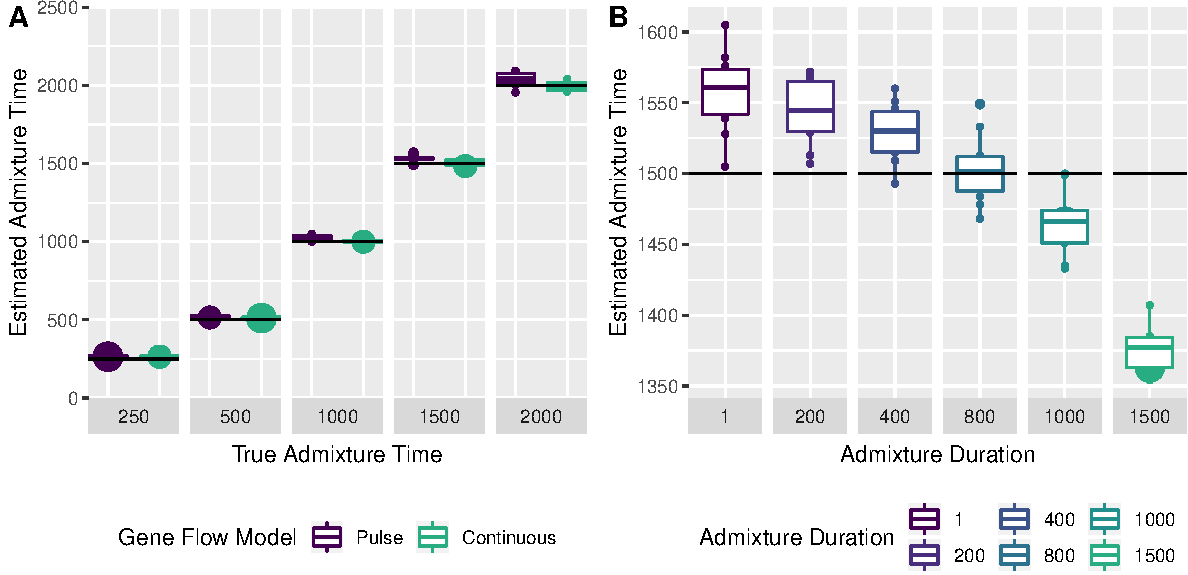
\includegraphics{Admixture_Time_Inference_Paper_Draft_files/figure-latex/fig2-1.pdf}
\caption{\label{fig:fig2} A) Comparison of mean admixture time estimates
between pulse and continuous gene flow for different admixture times.
The length of continuous gene flow corresponds to 50\% of the mean
admixture time, black line indicates true mean admixture time. B)
Comparison of mean admixture time estimates for simulations with a mean
time of admixture of 1500 generations ago, at a varying length of gene
flow. Boxplot created from 100 simulation replicates, respectively.}
\end{figure}


\subsection{Comparing effect sizes for technical covariates}\label{comparing effect sizes}

As the effect of ongoing gene flow is relatively minor, we next evaluate its relative importance for inference compared to other common assumptions made in the inference of admixture times. 

Therefore, we contrast the effect of extended gene flow on admixture time inference with  the effects of a complex demographic history and complex recombination map, as well as the impact of the ascertainment scheme and $d_0$ in the ALD estimation, using a simple and complex setting for each of these parameters. 

In Figure 3, we present the effect sizes of these four predictors on the admixture time inference. These effect sizes are estimated using a GLM (S. \ref{fig:figS2}) on simulations under all possible parameter combinations  (Supplement Table \ref{tab:tableS1}).

As a baseline, for comparison, we define a standard model as one using the LES ascertaiment, \(d_{0} = 0.05 cM\), simple demography and constant recombination map). 

As shown in the previous section, under the standard model admixture times are well-estimated, with a mean standardized difference of  -0.03 (-0.07 - 0.02 95 \% CI) from the true
admixture time.

We find that the  inclusion of a variable recombination map lead to a large underestimate of -1.47 -1.53 -- -1.42 $C.I._{95\%}$. In contrast, all other covariates had relatively moderate effect sizes. The extended pulse   (-0.24,  -0.29 -- -0.19) is in the range of biases arising from the ascertainment scheme (-0.33, -0.38 --
-0.28),a more complex demography (-0.25, -0.30 -- -0.20) and only slightly more then caused by a different $d_0$ (-0.20, -0.16 --
-0.26) (S.\ref{fig:figS2}).

Overall the bias introduced by the ascertainment, minimal distance
cutoff, demography and admixture model are  around +/-0.25 standard deviations or less. The major uncertainties in the admixture time
estimate arise from assuming a constant recombination rate. The
admixture time estimates for a simple or extended admixture pulse are similarly effected by the other modeling parameters.

\begin{figure}
\centering
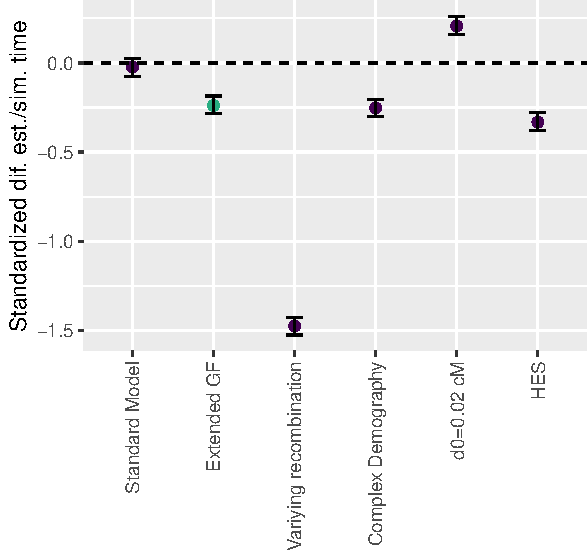
\includegraphics{Admixture_Time_Inference_Paper_Draft_files/figure-latex/fig3-1.pdf}
\caption{\label{fig:fig3} GLM effect size estimates for the parameters: admixture model (simple/extended), recombination rate (constant/varying), demography (simple/complex), minimal genetic distance (0.02/0.05 cM) and ascertainment scheme (LES/HES), on the standardized difference between simulated and estimated admixture time. Estimates are calculated across all possible combinations of parameters and are given as the estimate of the standard model pluse the respective parameter estimate. Dotted horizontal line indicates unbiased admixture estimates.}
\end{figure}


\subsection{Parameter estimation under the extended pulse model}\label{estimating the Lomax-parameters under different conditions}
In Figure \ref{fig:fig4}, we show the accuracy of $t_d$ and $t_m$ estimates in two sets of simulations. In panels A and B we increase both $t_m$ and $t_d$ at a similar rate, such that gene flow ends 50 generations before sampling ($t_{end}=50$, where $t_{end}= t_m - \frac{t_d}{2}$). In panels C and D $t_d$ is kept fixed at 800, but we increase $t_m$. We further vary recombination rate settings as i) inference and simulation under constant recombination rate, ii) simulation using HapMap, no correction, iii) simulation using HapMap, correction using AAMap, iv) inference and simulation using HapMap. 

Figure \ref{fig:fig4} A and C show the mean
time estimates received from the simple and extended pulse model fit. For simulations under a
constant recombination the mean time can be estimated confidently for different durations and different sampling times after the end of the admixture event in both cases. 

Under constant recombination settings, we find that parameters under the extended pulse are well-estimated in all scenarios, although we observe a small overestimate of both $t_m$ and $t_d$, for very long admixture durations in the very distant past. In contrast, inference under the simple pulse model results in a slight underestimate (Figure \ref{fig:fig2}, \ref{fig:fig4}).

We also find that the simple pulse model is fairly robust to changes in recombination settings, both using the ``correct'' and a empirically similar recombination map. Only when we do not correct for recombination rate variation, we observe a substantial underestimate by almost a factor of two for more distant admixture \ref{fig:fig4}. 

In contrast, estimates under the extended pulse model are substantially more spread out under variable recombination maps, but we do not observer the systematic bias towards more recent admxiture times as in the simple-pulse model. In contrast, the uncorrected scenario results in extremely poor estimates with very high variation, and is clearly unsuitable for this purpose \ref{fig:fig4}. 

We also find that estimates of $t_d$ differ substantially between recombination rate settings. Under constant rates, $t_d$ is well-estimated in all scenarios, and if the recombination rate is known, we get reasonably accurate estimates, at least if admixture is not very old. However, under the scenarios where recombination rates differ between simulation and inference, results become more erratic; For the cases of $t_d=200$ and $t_d=400$, many simulations infer an admixture time of near zero; in contrast, very old admixture results in a large overestimate.




\begin{figure}
\centering
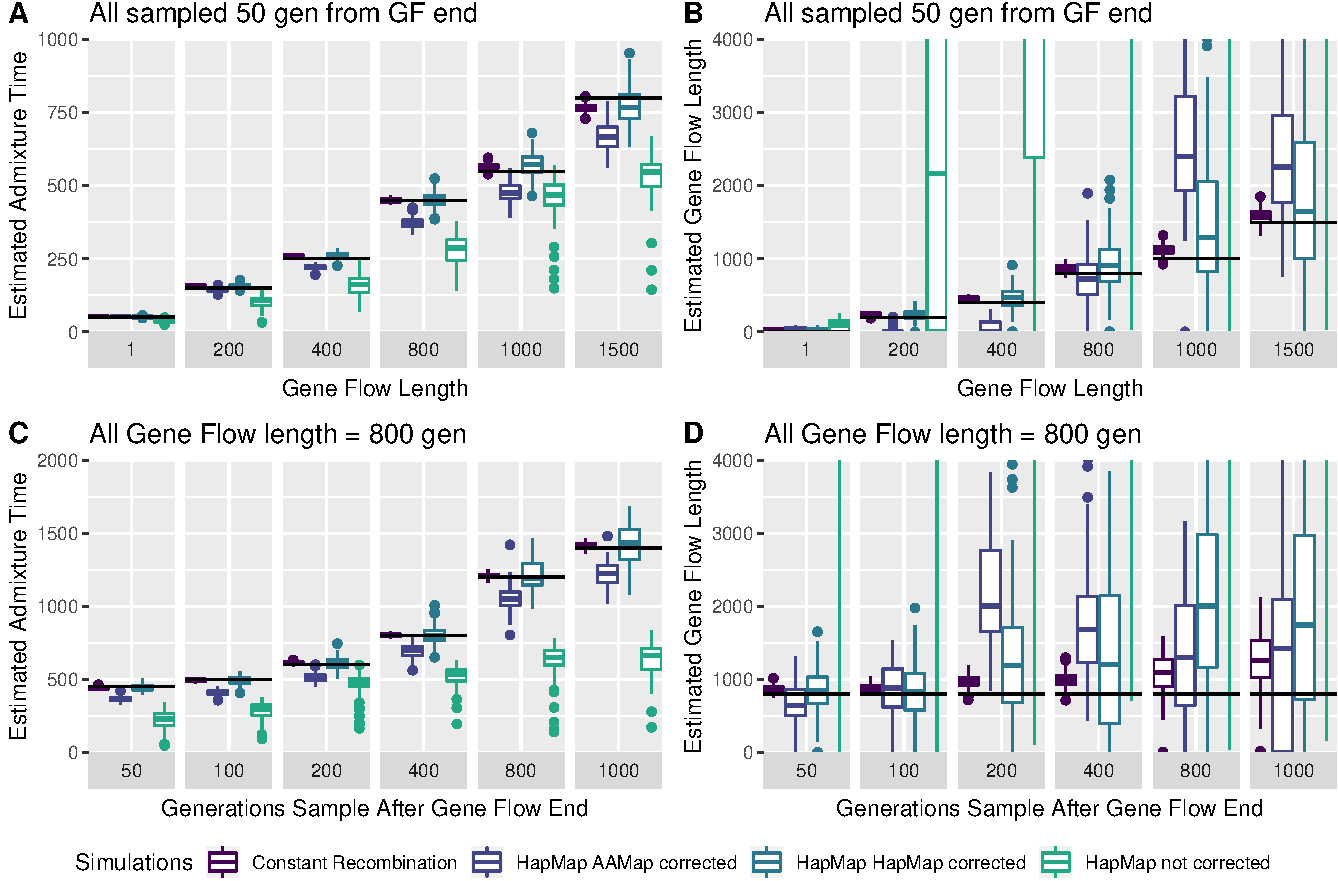
\includegraphics{Admixture_Time_Inference_Paper_Draft_files/figure-latex/fig4-1.pdf}
\caption{\label{fig:fig4} Comparison of parameter inference under the simple and extended pulse model  A) Mean time estimates $t_m$ for different gene
flow length all sampled 50 generations after the gene flow ended. B)
Duration estimate $t_d$ of the same scenario C) Mean time estimates for different sampling times after the end of 800
generations of gene flow. D) Duration estimate of the same scenario. All scenarious are simulated either under a constant recombination rate or an empirical (HapMap). Genetic distances for simulations under an empirical map are assigned by: assuming a constant rate, using a different map, using the same map.  }
\end{figure}

\subsection{Application to Neandertal data}
In the previous section, we have shown using simulations that it might be difficult to distinguish admixture scenarios of various durations particularly if it happened a long time ago. To evaluate that this is also true for real data, we aim to estimate the Neandretal admixture pulse from the 1000 genomes data, by fitting pulses of durations ranging from one generation up to 2,5000 generations to the ALD decay curve (
Figure \ref{fig:fig5}, S. Table \ref{tab:tableS2}). Plotting these best-fit ALD curves (Figure \ref{fig:fig5}A) on a y-axis in natural scale shows the extremely slight difference predicted under these drastically different gene flow scenarios. The difference between scenarios becomes more apparent if we log-transform the y-axis (\ref{fig:fig5}B), where we see that ongoing gene flow results in a heavier tail in the ALD distributions. However, due to finite size of the genome.




\begin{figure}
\centering
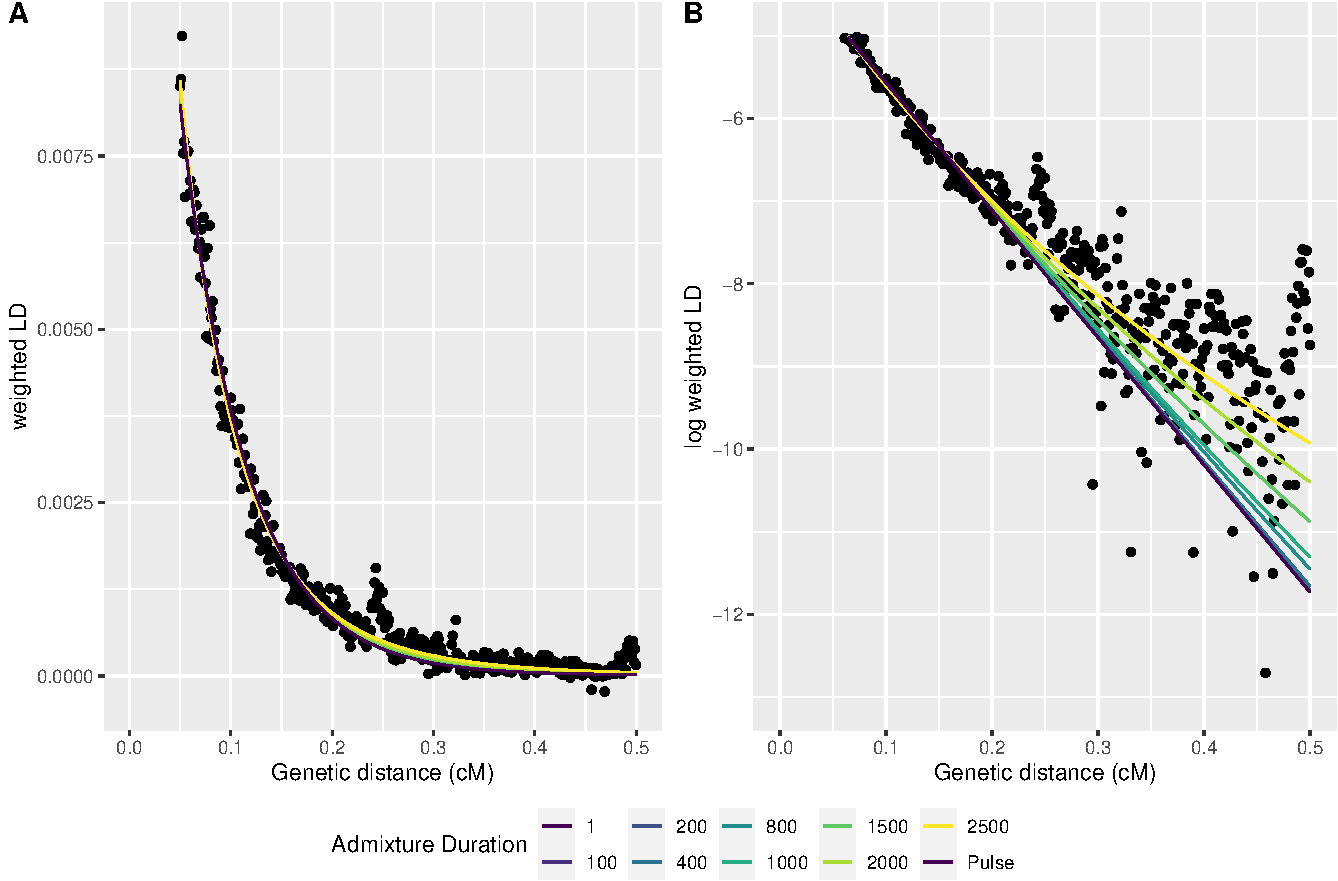
\includegraphics{Admixture_Time_Inference_Paper_Draft_files/figure-latex/fig5-1.pdf}
\caption{\label{fig:fig5} Different admixture duration models ranging
from a one generation pulse to 2500 generations of gene flow for Neandertal interbreeding using all 1k Genome CEU individuals as the admixed population
with all YRI and 3 high coverage Neandertals as reference populations. A) Weighted LD normal scaled B) Weighted LD log scaled.}
\end{figure}

\section{Discussion}\label{discussion}
While it is now well-established that early modern humans interbred with Neandertals, less consensus exists about when and where these interactions might have happened. Here we focus on genetic dating, one of the major approaches used to refine the plausible dates.

Previous estimates to date Neandertal-human gene flow have focused almost entirely on the mean time of gene flow, for which reasonably tight confidence intervals can be estimated \citep{green_draft_2010, sankararaman_date_2012}. Here, we show that these models cannot be used to establish bounds on when gene flow happened, as models involving hundreds of generations of gene flow are virtually indistinguishable from instantaneous gene flow. Thus, it is important to realize that the estimated time of gene flow of between 41 kya -- 54 kya \cite{moorjani_genetic_2016} is a confidence range for the mean time of gene flow, and does not bound when gene flow happened. This is of great practical importance as it might be tempting to link the genetic admixture date estimates with biogeographical events \citep{sankararaman_date_2012,lazaridis_genomic_2016,jacobs_multiple_2019,vyas_analyses_2019,douka_age_2019}. Indeed, our results show that substantial gene flow could also have happened tens of thousands of years before or after the mean time of gene flow. These dates are thus entirely consistent with early modern human genomes that have recent Neandertal ancestors \cite{fu_genome_2014, hajdinjak_bk_paper}. As we also show that mean time estimates are biased towards more recent dates, substantial gene flow might have happened before 54 kya. 

This is also important in the context of selection against Neandertal introgression \citep{harris_nielsen_2017, juric_plos_gen_2017}. 
READ UP ON THIS.

To further refine these dates, data from more early modern human and Neandertal genomes are likely needed. In particular, measures based on population differentiation (e.g \citep{browning_analysis_2018,wall_higher_2013,villanea_multiple_2019}) are very promising to understand the different events that contributed to archaic ancestry in present-day humans. While Neandertal ancestry in present-day people has been largely homogenized due to the substantial gene flow between populations, samples from both the Neandertal and early modern human populations immediately involved with the gene flow could likely refine when and where this gene flow happened. 


In addition, we show that particularly recombination rate variation has to be very carefully considered when making inferences about admixture times. This is because both an extended pulse, as well as a non-homogeneous recombination map, lead to an admixture track distribution that deviates from the expected exponential distribution. Correcting for just one of these factors may thus potentially conflate these issues, and may lead to a substantial underestimate of mean admixture times \cite{sankararaman_date_2012}. Therefore, accurate and population-specific fine-scale recombination maps are likely needed for accurate admixture time estimates, at least in the case for archaic admixture that happened more than a thousand generations ago; more recent admixture does appear to be somewhat more robust, perhaps because coarser-scale recombination maps are better estimated and differ less between populations \cite{hinch_landscape_2011}. 







Form our analyses using the extended model, we find that mean admixture time estimates vary little between models. However, we also show that even gene flow lasting thousands of generations may yield data that are practically indistinguishable from a one-generation pulse, and that other modelling and method assumptions have an impact on estimates that are of a similar magnitude or much higher. Particularly assumptions on the recombination rate are highly impactfull, and will lead to sever underestimations of admixture times. Therefore reliable mean time estimates can only be obtained using population specific recombination maps.




Here, we contrasted this pulse model with scenarios involving more long-standing gene flow.  Our model, assumes that migration rates  follow a Gamma distribution, which results in a simple closed-form expression for the introgressed segment lengths or ALD  distributions. 

In our analyses using the extended model, we find that mean admixture time estimates vary little between models. However, we also show that even gene flow lasting thousands of generations may yield data that are practically indistinguishable from a one-generation pulse, and that other modelling and method assumptions have an impact on estimates that are of a similar magnitude or much higher. Particularly assumptions on the recombination rate are highly impactfull, and will lead to sever underestimations of admixture times. Therefore reliable mean time estimates can only be obtained using population specific recombination maps.

The major implication of our result is that interpreting results of genetic dating is difficult.  Estimating the mean time of gene flow and its confidence intervals are not indicative of the actual duration of the interbreeding.  This is of great practical importance as it might be tempting to link the genetic admixture date estimates with biogeographical events \citep{sankararaman_date_2012,lazaridis_genomic_2016,jacobs_multiple_2019,vyas_analyses_2019,douka_age_2019}. For example, the lower bounds on admixture time estimates might be used as dates of Neandertal extinction, and likewise use the earliest dates of gene flow as evidence when the out-of-Africa migration happened \citep{sankararaman_date_2012}. Our results show that both of these interpretations might be misleading. However, using the extended pulse model relaxing the one generation pulse assumptions used for earlier estimates, also indicates that most of the gene flow was around 45,000 to 65,000 years ago, consistent with previous estimates.


While our results show that drawing concrete conclusions from admixture time estimates can be misleading, other avenues for differentiating different gene flow events remain fruitful.
In particular, measures based on population differentiation (e.g \citep{browning_analysis_2018,wall_higher_2013,villanea_multiple_2019}) are very promising to understand the different events that contributed to archaic ancestry in present-day humans. 

The other major avenue are ancient DNA samples from early modern humans that lived around or immediately after gene flow between archaic and modern humans occurred. The \textit{Oase 1} \citep{fu_genome_2014} genome is a prime example, as it directly demonstrates that some gene flow must have occurred in Europe, around 40,000 years ago, concurrently with when \textit{Oase 1} lived. More generally, detailed analyses of ancient genomes from the initial upper paleolithic should provide more accurate mean dates, as they are much closer to the gene flow, and may give better evidence about the duration of the gene flow. The drawback is that some of the gene flow these individuals experience may be private to their population, as has e.g. been suggested for \textit{Oase 1}. Larger numbers of early modern human genomes, as well as methods to accurately infer admixture tracts or ALD in low-coverage data will likely enable this line of research. 


\hypertarget{refs}{}

\bibliography{References/MyLibraryATE}


\pagebreak
\setcounter{figure}{0} \renewcommand{\figurename}{Fig. S}
\renewcommand{\tablename}{Tab. S}

\section{Supplement}\label{supplement}

\subsection{Extended Pulse Model}

In this section, we describe in detail the derivation of the extended pulse model, where the gene flow over time is modeled as a Gamma distribution with shape parameter $k$ and scale parameter $\frac{k}{t_m}$. Here, $L_i$ is the length of a segment entered at time $T_i$. We assume each segment length at time $T_i$ to be described by an exponential distribution (eq. \ref{eq:generall_length_distribution}).

To get the likelihood function for the segment length distribution $P(L_i)$ under the extended pulse we have to solve the following integral:

\begin{equation}
\label{eq:Likelihood_function_extended_pulse_1}
    P(L_i=l) = \int_{0}^{\infty} \frac{1}{\Gamma(k)(\frac{t_m}{k})^k}t^{k-1}e^{-t\frac{k}{t_m}}\ t\ e^{-tl} \ dt 
\end{equation}

we can factor out all terms not depending on $t$:

\begin{equation}
\label{eq:Likelihood_function_extended_pulse_2}
    P(L=l) = \frac{1}{\Gamma(k)(\frac{t_m}{k})^k}\ \int_{0}^{\infty}\ t^{k-1}e^{-t\frac{k}{t_m}}\ t\ e^{-tl} \ dt 
\end{equation}

 
we can re-write the integral into the  form of the known integral $\int_{0}^{\infty}\ x^n e^{-\alpha x} \ dx= \frac{\Gamma{n+1}}{\alpha^{n+1}}$

\begin{equation}
\begin{split}
\label{eq:Likelihood_function_extended_pulse_3}
    P(L=l) &= \frac{1}{\Gamma(k)(\frac{t_m}{k})^k}\ \int_{0}^{\infty}\ t^{k}e^{-(l+\frac{k}{t_m})t} \ dt \\ 
    P(L=l) &= \frac{1}{\Gamma(k)(\frac{t_m}{k})^k}\ \frac{\Gamma(k+1)}{l+\frac{k}{t_m})^{k+1}} 
\end{split}
\end{equation}

since $\frac{\Gamma(k+1)}{\Gamma(k)} =k$ we can re-write the likelihood to:



\begin{equation}
\begin{split}
\label{eq:Likelihood_function_extended_pulse_final}
    P(L=l) &= \frac{k}{(\frac{t_m}{k})^k \ (l+\frac{k}{t_m})^{k+1}} \\
    &= \frac{k(\frac{k}{t_m})^k} {(l+\frac{k}{t_{m}})^{k+1}}  \\
    &= \frac{k^{k+1}} { t_{m}^k \ (l+\frac{k}{t_{m}})^{k+1}}  \\
    &= t_{m} \ \Bigg( \frac{k}{t_{m}(l+\frac{k}{t_{m}})}\Bigg)^{k+1} \\
    P(L=l) &= t_{m}^{-k} \ \Bigg( \frac{k}{(l+\frac{k}{t_{m}})}\Bigg)^{k+1}
\end{split}
\end{equation}


\subsection{Supplement Figures }

\begin{figure}
\centering
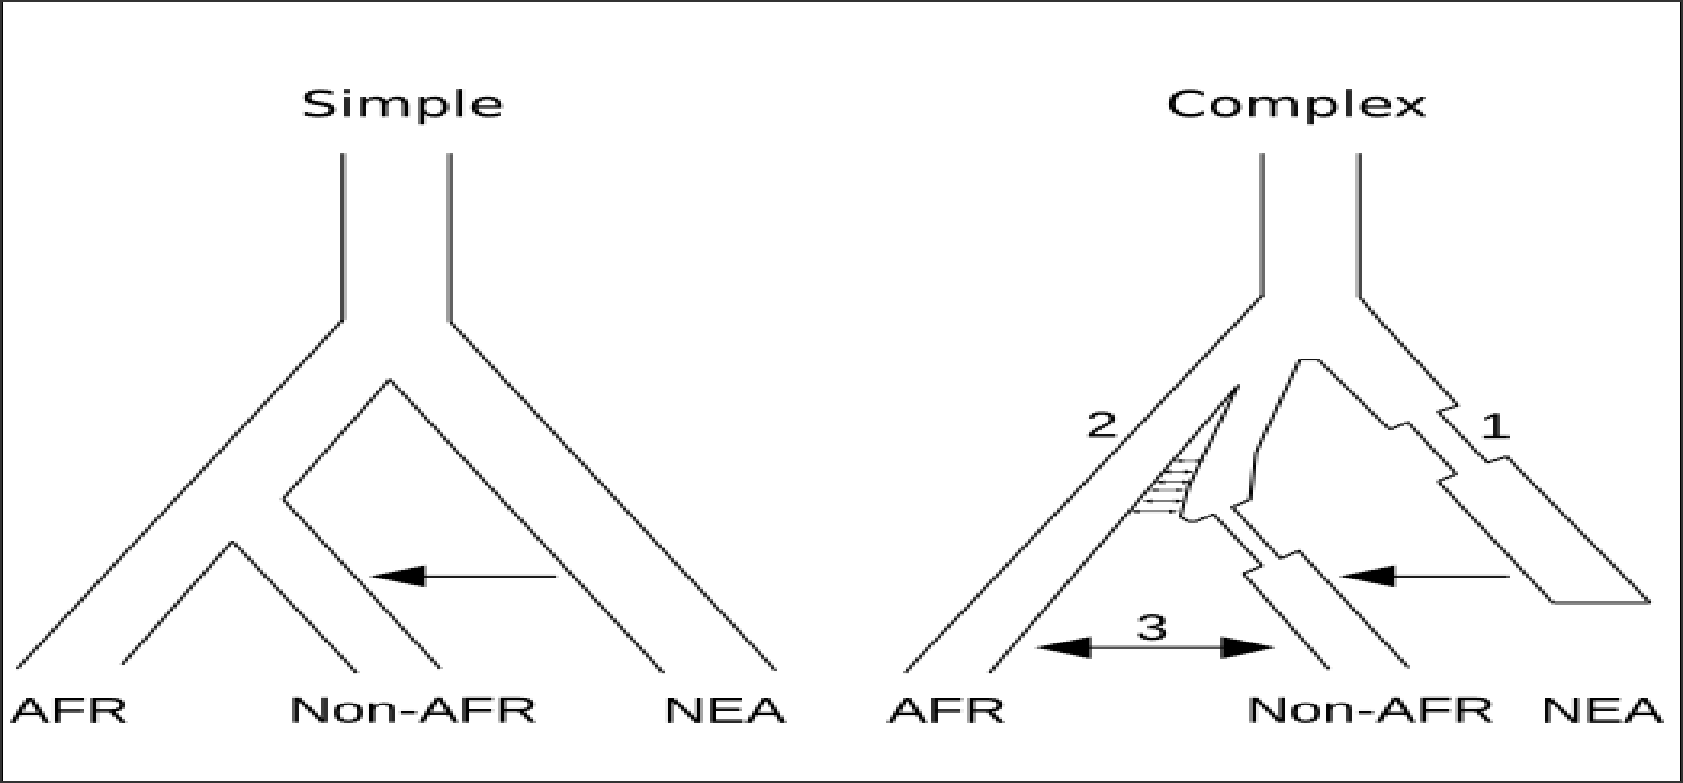
\includegraphics{Admixture_Time_Inference_Paper_Draft_files/figure-latex/figS1-1.pdf}
\caption{\label{fig:figS1} Demographic models of Neandertal admixture with non-Africans used for the simulations. A) Simple demographic model used for ALD simulations with constant population sizes. B) Complex demographic model with substructure in Africa, where after an initial earlier split and isolation the structured population exchange migrants till the final split and additional gene flow between Africans and non-Africans after the Neandertal admixture. The  population sizes after the (final) split are taken fome MSMC/PSMC estimates for the respective populations. C) Demographic model for the direct inference of Neandertal segments in non-Africans taken and modified from Skov et al. 2018. (\citep{skov_detecting_2018})}
\end{figure}

\begin{figure}
\centering
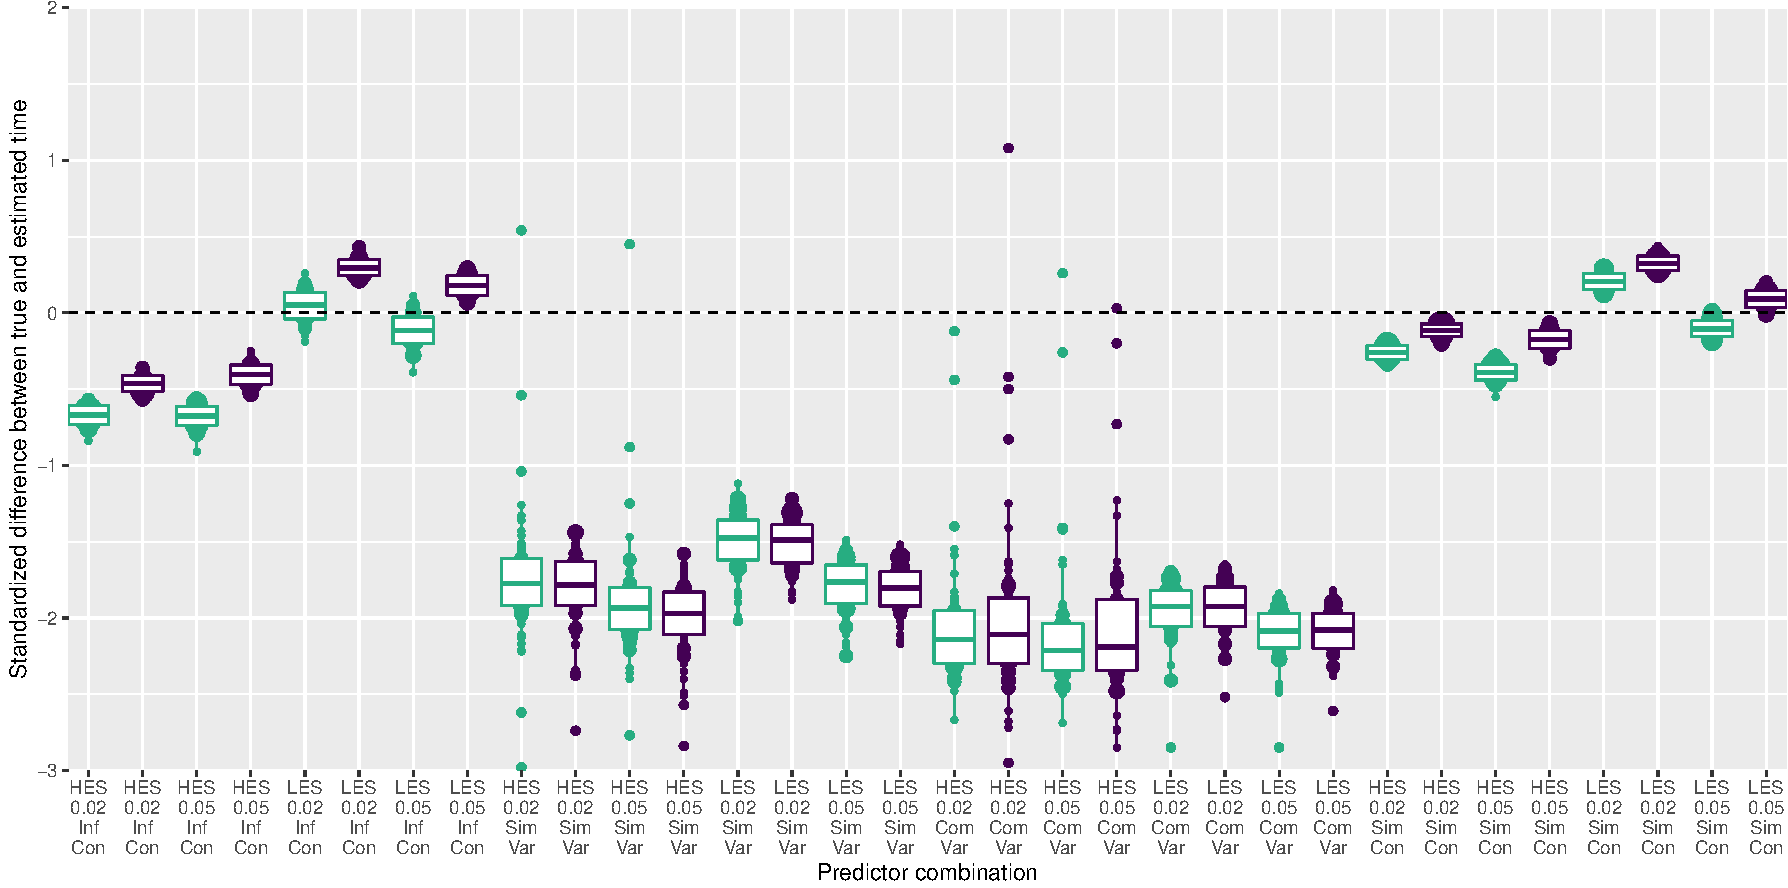
\includegraphics{Admixture_Time_Inference_Paper_Draft_files/figure-latex/figS2-1.pdf}
\caption{\label{fig:figS2} Comparison of the standardized difference between true and estimated admixture time for all combinations of parameters: ascertainment scheme = LES/HES,  $d_{0}$ = 0.02/0.05 cM, demography = simple/complex, recombination = constant/variable and the gene flow model = pulse/continuous, with 100 replicates respectively. Dotted horizontal line indicates no difference between true and estimated time.}
\end{figure}

\begin{table}[H]

\caption{\label{tab:tableS1}\label{tab:tableS1} Mean, standart deviation, 5.5/94.5 compatibility interval of the posterior distribution for every parameter effect on the standardized difference between true and estimated admixture time.}
\centering
\begin{tabular}{l|r|r|r|r|r|r}
\hline
  & mean & sd & 5.5\% & 94.5\% & n\_eff & Rhat\\
\hline
a & 0.12 & 0.02 & 0.08 & 0.16 & 1220.94 & 1\\
\cline{1-7}
bG & -0.31 & 0.02 & -0.34 & -0.28 & 1559.84 & 1\\
\cline{1-7}
bR & -1.73 & 0.02 & -1.76 & -1.70 & 2112.69 & 1\\
\cline{1-7}
bD & -0.22 & 0.02 & -0.25 & -0.19 & 2036.66 & 1\\
\cline{1-7}
bm & 0.13 & 0.02 & 0.10 & 0.17 & 1657.66 & 1\\
\cline{1-7}
bA & -0.32 & 0.02 & -0.35 & -0.29 & 1721.62 & 1\\
\cline{1-7}
sigma & 0.46 & 0.01 & 0.44 & 0.47 & 2239.47 & 1\\
\hline
\end{tabular}
\end{table}

\begin{figure}
\centering
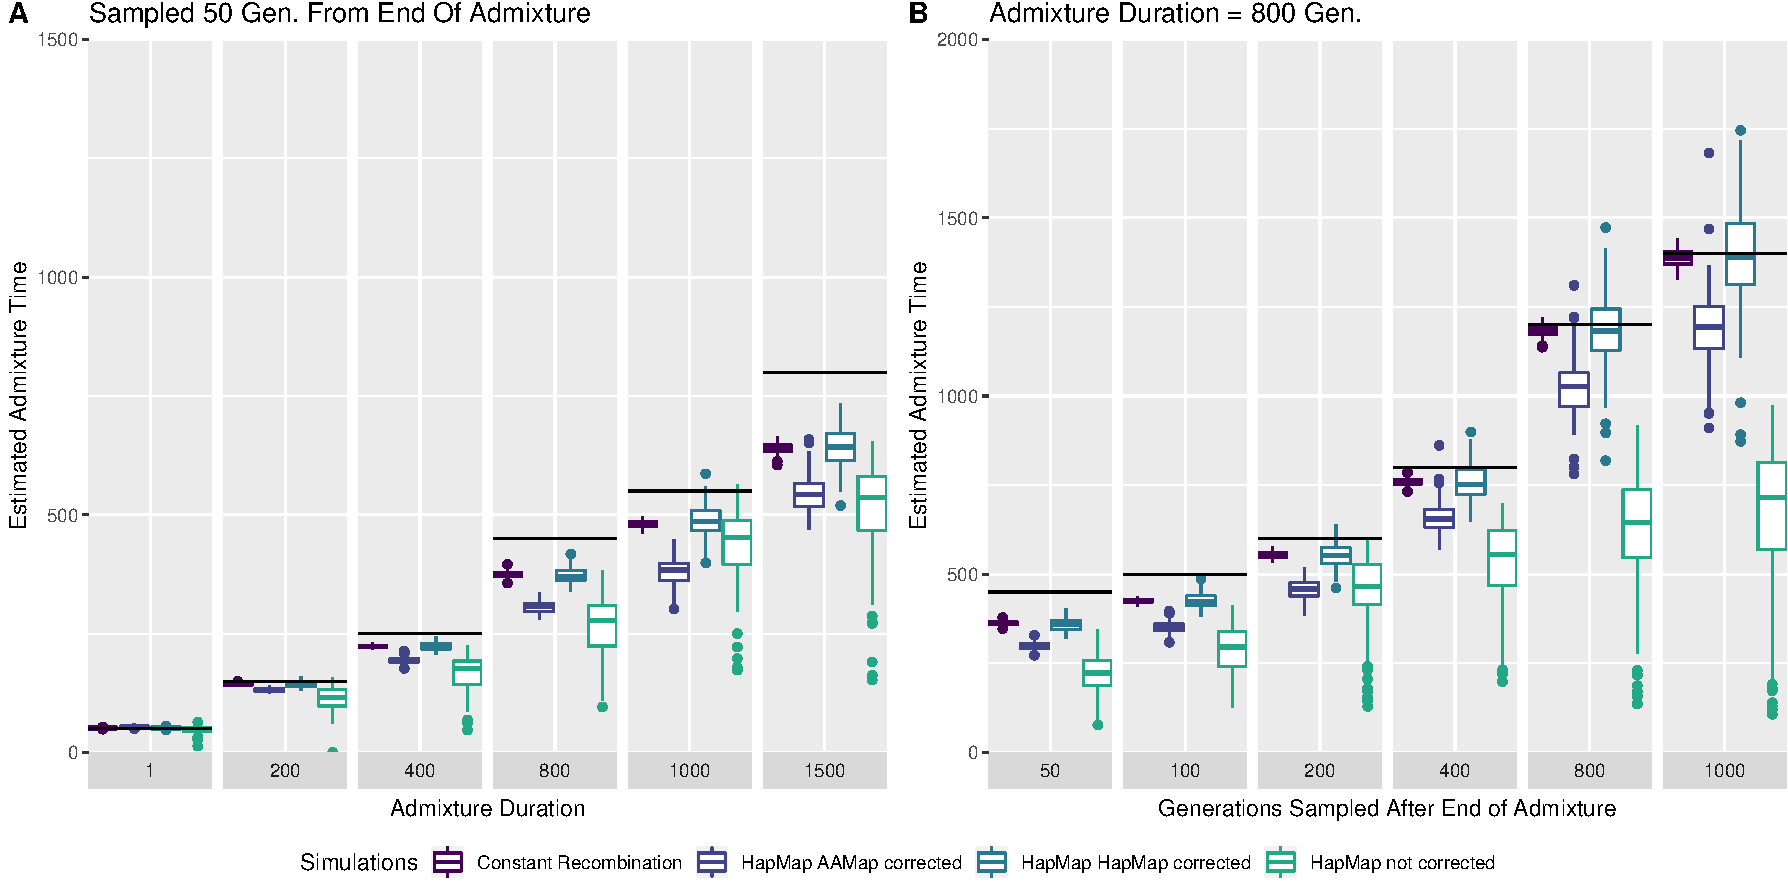
\includegraphics{Admixture_Time_Inference_Paper_Draft_files/figure-latex/figS3-1.pdf}
\caption{\label{fig:figS3} Mean time estimates of the Exponential model A) Mean time estimates for different 
admixture durations all sampled 50 generations after the admixture ended. B) Mean time estimates for different sampling times after the end of 800
generations of continuous admixture.}
\end{figure}

\subsection{Supplement Tables}

\begin{table}[H]
\caption{\label{tab:tableS2}\label{tab:tableS2} Mean and 2.5/97.5 compatibility interval for every parameter estimated in the model fit}
\centering
\begin{tabular}{l|l|l|l|l}
\hline
Model & Parameter & Estimate & 2.5 \% & 97.5 \%\\
\hline
Exponential & A & 0.0177951442439937 & 0.0177907714786252 & 0.0177995170093623\\
\hline
Exponential & mean time & 1540.51741259424 & 1486.87051449324 & 1598.18041766271\\
\hline
Exponential & c & 1.04922402241663e-05 & 6.11947485562607e-06 & 1.48650055927066e-05\\
\hline
Lomax (td=1) & A & 0.0177951442439937 & 0.0177907714786252 & 0.0177995170093623\\
\hline
Lomax (td=1) & mean time & 1540.54690341371 & 1486.89897832594 & 1598.21101235108\\
\hline
Lomax (td=1) & c & 1.04949518630901e-05 & 6.12218649454983e-06 & 1.48677172316303e-05\\
\hline
Lomax (td=100) & A & 0.0177951442439937 & 0.0177907714786252 & 0.0177995170093623\\
\hline
Lomax (td=100) & mean time & 1541.21552745233 & 1487.54431823588 & 1598.90466361173\\
\hline
Lomax (td=100) & c & 1.04778971116211e-05 & 6.10513174308087e-06 & 1.48506624801614e-05\\
\hline
Lomax (td=200) & A & 0.0177951442439937 & 0.0177907714786252 & 0.0177995170093623\\
\hline
Lomax (td=200) & mean time & 1543.30241011905 & 1489.55852740936 & 1601.0696602451\\
\hline
Lomax (td=200) & c & 1.04341296352963e-05 & 6.06136426675609e-06 & 1.48068950038366e-05\\
\hline
Lomax (td=400) & A & 0.0177951442439937 & 0.0177907714786252 & 0.0177995170093623\\
\hline
Lomax (td=400) & mean time & 1551.70459843938 & 1497.66811836146 & 1609.78635031902\\
\hline
Lomax (td=400) & c & 1.02583870973029e-05 & 5.88562172876263e-06 & 1.46311524658431e-05\\
\hline
Lomax (td=800) & A & 0.0177951442439937 & 0.0177907714786252 & 0.0177995170093623\\
\hline
Lomax (td=800) & mean time & 1586.19945700954 & 1530.96172977427 & 1645.57238365183\\
\hline
Lomax (td=800) & c & 9.54350178205991e-06 & 5.17073641351966e-06 & 1.39162671506002e-05\\
\hline
Lomax (td=1000) & A & 0.0177951442439937 & 0.0177907714786252 & 0.0177995170093623\\
\hline
Lomax (td=1000) & mean time & 1613.04056713235 & 1556.86812647683 & 1673.41818158693\\
\hline
Lomax (td=1000) & c & 8.99447037087496e-06 & 4.62170500233471e-06 & 1.33672357394152e-05\\
\hline
Lomax (td=1500) & A & 0.0177951442439937 & 0.0177907714786252 & 0.0177995170093623\\
\hline
Lomax (td=1500) & mean time & 1713.23411309364 & 1653.57253761458 & 1777.36206551997\\
\hline
Lomax (td=1500) & c & 6.99221511836012e-06 & 2.61944974981987e-06 & 1.13649804869004e-05\\
\hline
Lomax (td=2000) & A & 0.0177951442439937 & 0.0177907714786252 & 0.0177995170093623\\
\hline
Lomax (td=2000) & mean time & 1874.70574615156 & 1809.42109093705 & 1944.87773256239\\
\hline
Lomax (td=2000) & c & 3.90606333903974e-06 & -4.66702029500504e-07 & 8.27882870757999e-06\\
\hline
Lomax (td=2500) & A & 0.0177951442439937 & 0.0177907714786252 & 0.0177995170093623\\
\hline
Lomax (td=2500) & mean time & 2128.77896518946 & 2054.64647743473 & 2208.46114940615\\
\hline
Lomax (td=2500) & c & -6.57497391994452e-07 & -5.0302627605347e-06 & 3.7152679765458e-06\\
\hline
\end{tabular}
\end{table}



\end{document}